\documentclass[compress,svgnames,xcolor=table]{beamer}
\mode<presentation>

% Include additional LaTeX packages
\usepackage{etex}
\usepackage{pifont}
\usepackage{multicol}
\usepackage{amsmath}
\usepackage{epsfig}
\usepackage{pgfplots}
\usepackage{graphicx}
\usepackage[all,knot]{xy}
\xyoption{arc}
\usepackage{url}
\usepackage{multimedia}
\usepackage{hyperref}
\usepackage{setspace}
\usepackage{listings}
\usepackage{tikz}
\usetikzlibrary{positioning}
\usepackage{threeparttable}


\definecolor{lightgray}{gray}{.95}
\definecolor{darkgray}{gray}{.80}

% Set up Beamer theme
\usetheme{Dresden}
\usecolortheme{lily}
\usefonttheme{structuresmallcapsserif}
\usepackage{beamerinnerthemecircles}
\usepackage{beamerouterthememiniframes}
\useoutertheme[subsection=false]{smoothbars}

% Removes the Beamer navigation symbols
\setbeamertemplate{navigation symbols}{}

% Sets the color for the \alert{} text
\setbeamercolor{alerted text}{fg=blue}

% Presentation information
\title[RAISE 2012 -- \insertframenumber/\inserttotalframenumber]{Predicting Mutation Score Using Source Code and Test Suite Metrics \vspace{2mm} \hrule}
\subtitle{RAISE 2012}
\author[\copyright 2012, Kevin Jalbert and Jeremy S. Bradbury]{\textbf{Kevin Jalbert} and Jeremy S. Bradbury}
\institute[UOIT]{University of Ontario Institute of Technology}
\date{\tiny June 5$^{th}$, 2012}

\begin{document}

% Create title page
\frame{\maketitle}

\section{Overview}
\frame{
  \setcounter{tocdepth}{2}
  \tableofcontents[currentsection,hideothersubsections]
}

\subsection{Problem}
\frame{\frametitle{Problem}
  \begin{itemize}
    \item Mutation testing is an \alert{effective} yet \alert{costly} coverage technique
      \begin{itemize}
        \item A \alert{fault}-based \alert{coverage} technique
        \item Closest measure to \alert{test suite effectiveness}
      \end{itemize}
    \item Mutation testing would have to be applied \alert{frequently} during development
  \end{itemize}
}

\subsection{Our Solution}
\frame{\frametitle{Our Solution}
  \begin{quote}
  \Large
  \centering
    ``Our proposed approach uses machine learning to predict the mutation score based on a combination of source code and test suite metrics of the code unit under test''
  \end{quote}
  \vspace{5mm}
  \hrule
  \vspace{5mm}
  \begin{itemize}
    \item A \alert{``do fewer and smarter''} technique
    \begin{itemize}
      \item Indicate source code units that have \alert{low coverage}
      \item Ability to \alert{prioritize} mutation testing for specific mutants
    \end{itemize}
  \end{itemize}
}

\subsection{Our Approach}
\frame{\frametitle{Our Approach}
  \begin{itemize}
    \item Collect \alert{feature data} for source code units
    \begin{itemize}
      \item Source code metrics
      \item Test suite metrics
    \end{itemize}
    \item Collect \alert{category data} for source code units
      \begin{itemize}
        \item Mutation score for source code units
      \end{itemize}
    \item \alert{Train} and \alert{predict} using Support Vector Machine (SVM)
  \end{itemize}
}

\section{Background}
\frame{
  \setcounter{tocdepth}{2}
  \tableofcontents[currentsection,hideothersubsections]
}

\subsection{Mutation Testing}
\frame{\frametitle{Mutation Testing}
  \centering
  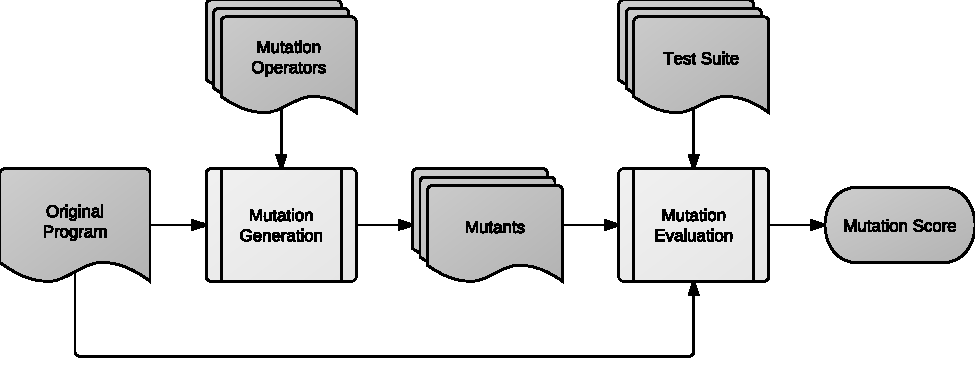
\includegraphics[width=8cm]{figures/mutation_testing_overview.pdf}
  \vspace{2mm}
  \begin{itemize}
    \item Create \alert{mutants} from original program using \alert{mutation operators}
    \item Compare mutant's \alert{results} against original program using \alert{test suite}
    \item Mutation score is \alert{percent} of non-equivalent mutants \alert{killed}
  \end{itemize}
}

\subsection{Support Vector Machine}
\frame{\frametitle{Support Vector Machine}
  \begin{itemize}
    \item A \alert{supervised} machine learning \alert{classification} technique
    \item Models a \alert{feature space} is constructed using a \alert{set of vectors}
    \item Each \alert{vectors} has a set of \alert{attributes} and a \alert{category}
    \item Attempts to \alert{linearly separate} vectors
  \end{itemize}
  \begin{figure}
    \centering
    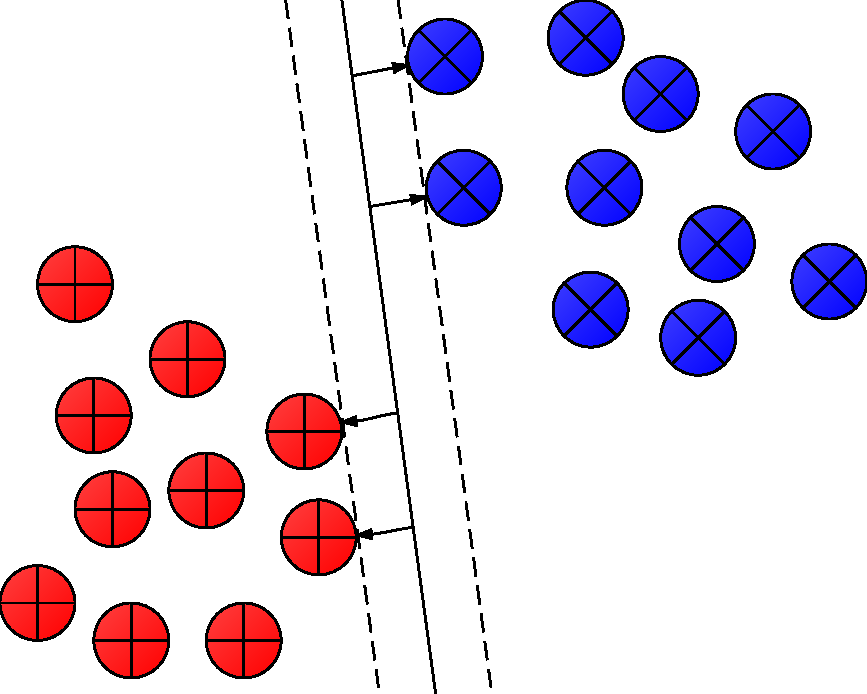
\includegraphics[width=3.5cm]{figures/SVM_small_margin.pdf}
    $\xrightarrow{\texttt{Better Margin}}$
    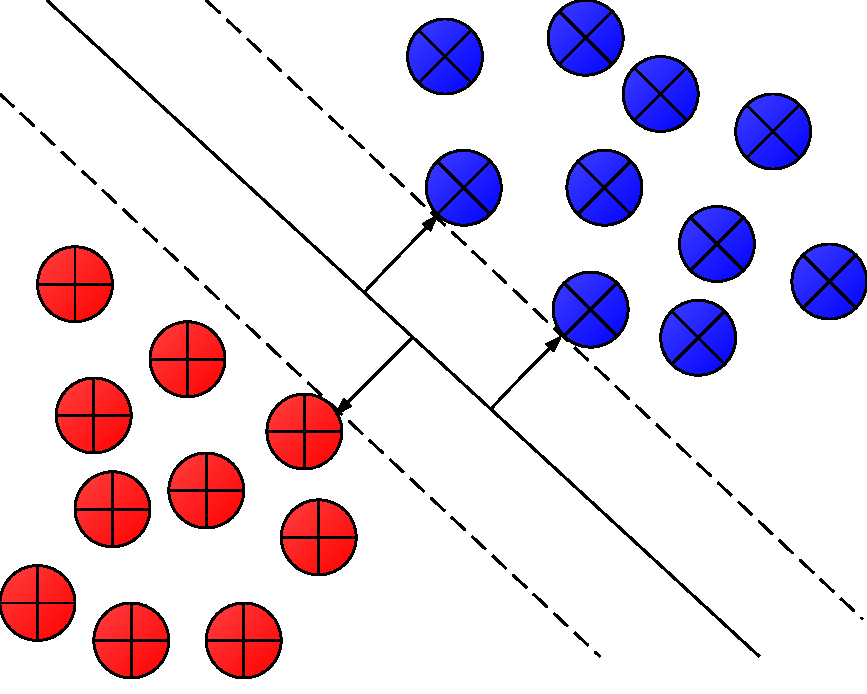
\includegraphics[width=3.5cm]{figures/SVM_maximum_margin.pdf}
  \end{figure}
}

\subsubsection{Support Vector Machine -- cont.}
\frame{\frametitle{Support Vector Machine -- cont.}
  \begin{itemize}
    \item Can work for \alert{\emph{many}-group} classification
    \item Can work on \alert{non-linearly separable} data using \alert{kernel functions}
  \end{itemize}
  \begin{figure}
    \centering
    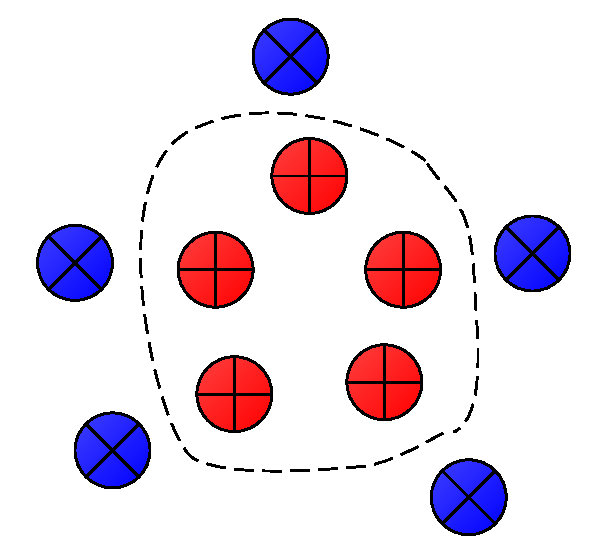
\includegraphics[width=3.5cm]{figures/SVM_non-linear.pdf}
    $\xrightarrow{\texttt{Kernel Function}}$
    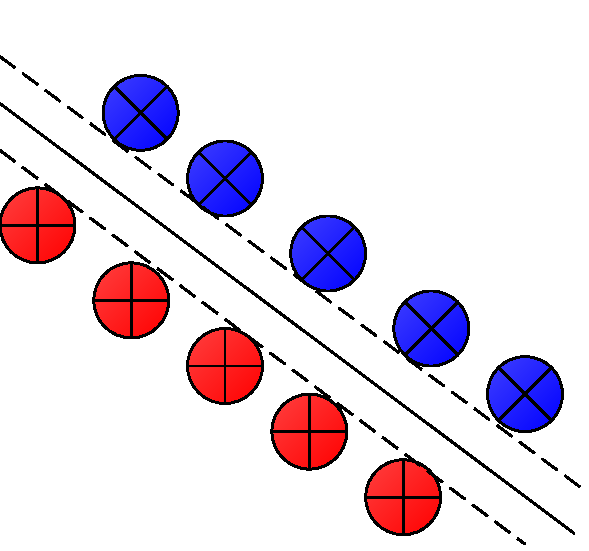
\includegraphics[width=3.5cm]{figures/SVM_kernel_function.pdf}
  \end{figure}
}

\subsection{Metrics}
\frame{\frametitle{Metrics}
  \begin{itemize}
    \item \alert{Measurements} that describe \alert{structural} and \alert{behavioral} \alert{properties} of a software system
    \item We use \alert{four sets} of software metrics
    \begin{itemize}
      \item Source Code Metrics
      \item Accumulated Source Code Metrics
      \item Coverage Metrics
      \item Accumulated Test Case Metrics
    \end{itemize}
  \end{itemize}
}

\section{Process}
\frame{
  \setcounter{tocdepth}{2}
  \tableofcontents[currentsection,hideothersubsections]
}

\subsection{Data Collection}
\frame{\frametitle{Data Collection}
  \begin{figure}
    \begin{minipage}{5.25cm}
      \begin{itemize}
        \item \alert{Input}: Units of test cases and units of source code
        \begin{enumerate}
          \item Collect \alert{mutation scores} using \texttt{Javalanche}
          \item Collect \alert{source code metrics} using \texttt{Eclipse Metrics Plugin}
          \item Collect \alert{coverage} metrics using \texttt{EMMA}
        \end{enumerate}
      \end{itemize}
    \end{minipage}
    \hfill
    \begin{minipage}{5.25cm}
      \flushright
      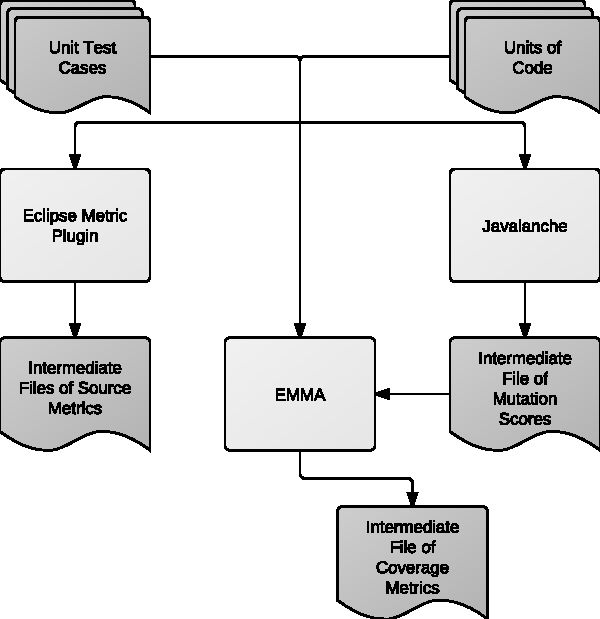
\includegraphics[width=5.25cm]{figures/process_part1.pdf}
      \vspace{-5mm}
      \Huge \centering
      \ldots
    \end{minipage}
  \end{figure}
}

\subsubsection{Mutation Operators}
\frame{\frametitle{Mutation Operators}
  \begin{table}[h]
    \centering
    \rowcolors{2}{gray!30}{gray!20}
    \begin{tabular}{|l|l|}
      \hline
      \rowcolor[RGB]{169,196,223}
      \textbf{Name} & \textbf{Description} \\
      \hline REPLACE\_CONSTANT & Replace a constant \\
      \hline NEGATE\_JUMP & Negate jump condition \\
      \hline ARITHMETIC\_REPLACE & Replace arithmetic operator \\
      \hline REMOVE\_CALL & Remove method call \\
      \hline REPLACE\_VARIABLE & Replace variable reference\\
      \hline ABSOLUTE\_VALUE & Insert absolute value of a variable \\
      \hline UNARY\_OPERATOR & Insert unary operator \\
      \hline
    \end{tabular}
  \end{table}
  \begin{itemize}
    \item Set of selective method-level mutation operators used in \texttt{Javalanche}.
  \end{itemize}
}

\subsubsection{Source Code Metrics}
\frame{\frametitle{Source Code Metrics}
  \begin{table}
    \small
    \centering
    \rowcolors{2}{gray!30}{gray!20}
    \begin{tabular}{|l|l|l|}
      \hline
      \rowcolor[RGB]{169,196,223}
      \textbf{Metrics} & \textbf{Description} & \textbf{Scope} \\
      \hline MLOC & Method lines of code & Method \\
      \hline NBD & Nested block depth & Method \\
      \hline VG & McCabe cyclomatic complexity & Method \\
      \hline PAR & Number of parameters & Method \\
      \hline NORM & Number of overridden methods & Class \\
      \hline NOF & Number of attributes & Class \\
      \hline NSC & Number of children & Class \\
      \hline DIT & Depth of inheritance tree & Class \\
      \hline LCOM & Lack of cohesion of methods & Class \\
      \hline NSM & Number of static methods & Class \\
      \hline NOM & Number of methods & Class \\
      \hline SIX & Specialization index & Class \\
      \hline WMC & Weighted method per class & Class \\
      \hline NSF & Number of static attributes & Class \\
      \hline
    \end{tabular}
  \end{table}
}

\subsubsection{Accumulated Source Code Metrics}
\frame{\frametitle{Accumulated Source Code Metrics}
  \begin{table}
    \small
    \centering
    \rowcolors{2}{gray!30}{gray!20}
    \begin{tabular}{|l|l|l|}
      \hline
      \rowcolor[RGB]{169,196,223}
      \textbf{Metrics} & \textbf{Description} & \textbf{Scope} \\
      \hline SMLOC & Sum MLOC of methods & Class \\
      \hline SNBD & Sum NBD of methods & Class \\
      \hline SVG & Sum VG of methods & Class \\
      \hline SPAR & Sum PAR of methods & Class \\
      \hline AMLOC & Average MLOC of methods & Class \\
      \hline ANBD & Average NBD of methods & Class \\
      \hline AVG & Average VG of methods & Class \\
      \hline APAR & Average PAR of methods & Class \\
      \hline
    \end{tabular}
  \end{table}
}

\subsubsection{Coverage Metrics}
\frame{\frametitle{Coverage Metrics}
  \begin{table}
    \small
    \centering
    \rowcolors{2}{gray!30}{gray!20}
    \begin{tabular}{|l|l|l|}
      \hline
      \rowcolor[RGB]{169,196,223}
      \textbf{Metrics} & \textbf{Description} & \textbf{Scope} \\
      \hline BCOV & Basic blocks covered in code unit & Class/Method \\
      \hline BTOT & Total basic blocks for code unit & Class/Method \\
      \hline
    \end{tabular}
  \end{table}
}

\subsubsection{Accumulated Test Case Metrics}
\frame{\frametitle{Accumulated Test Case Metrics}
  \begin{table}
    \small
    \centering
    \rowcolors{2}{gray!30}{gray!20}
    \begin{tabular}{|l|l|l|}
      \hline
      \rowcolor[RGB]{169,196,223}
      \textbf{Metrics} & \textbf{Description} & \textbf{Scope} \\
      \hline STMLOC & Sum MLOC of test methods & Class/Method \\
      \hline STNBD & Sum NBD of test methods & Class/Method \\
      \hline STVG & Sum VG of test methods & Class/Method \\
      \hline STPAR & Sum PAR of test methods & Class/Method \\
      \hline ATMLOC & Average MLOC of test methods & Class/Method \\
      \hline ATNBD & Average NBD of test methods & Class/Method \\
      \hline ATVG & Average VG of test methods & Class/Method \\
      \hline ATPAR & Average PAR of test methods & Class/Method \\
      \hline
    \end{tabular}
  \end{table}
}

\subsection{Data Synthesis}
\frame{\frametitle{Data Synthesis}
  \begin{figure}
    \begin{minipage}{5.25cm}
      \begin{itemize}
        \item \alert{Goal}: Category/feature data for source code units
        \begin{enumerate}
          \item \alert{Combine} source code and coverage metrics together
          \item \alert{Merge} source code metrics of the \alert{touched tests} for each source code unit
          \item \alert{Aggregate method-level} source code unit metrics into \alert{class-level} source code units
          \item \alert{Create \texttt{.libsvm}} file using feature/category data
        \end{enumerate}
      \end{itemize}
    \end{minipage}
    \hfill
    \begin{minipage}{5.25cm}
      \Huge \centering
      \ldots
      \vspace{-2mm}
      \flushright
      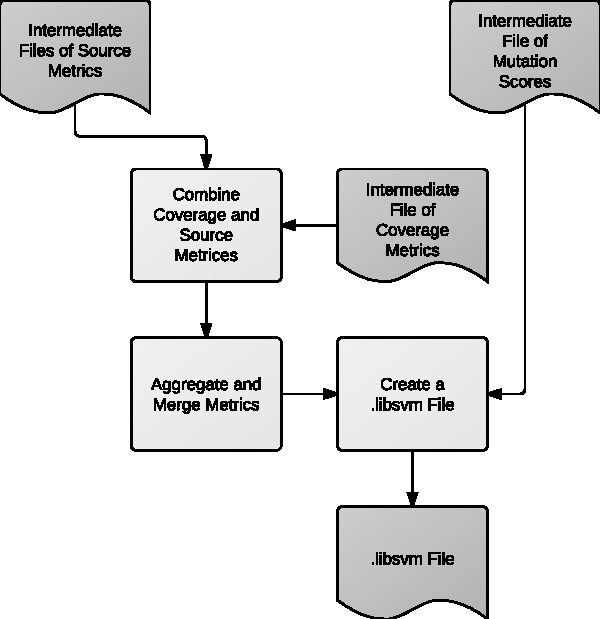
\includegraphics[width=5.25cm]{figures/process_part2.pdf}
    \end{minipage}
  \end{figure}
}

\subsection{.libsvm File}
\frame{\frametitle{.libsvm File}
  \begin{minipage}{\linewidth}
    \scriptsize
    \lstinputlisting{listings/libsvm_example.libsvm}
  \end{minipage}
  \begin{itemize}
    \item \texttt{LIBSVM} requires a \alert{specific} file format
    \begin{itemize}
      \item \texttt{category attribute\_1:value attribute\_2:value \ldots}
    \end{itemize}
    \item We have \alert{class} and \alert{method} \texttt{.libsvm} file
  \end{itemize}
}

\section{Results}
\frame{
  \setcounter{tocdepth}{2}
  \tableofcontents[currentsection,hideothersubsections]
}

\subsection{Case Study -- JGAP}
\frame{\frametitle{Case Study -- JGAP}

  \begin{table}
  \begin{threeparttable}
    \centering
    \rowcolors{2}{gray!30}{gray!20}
    \begin{tabular}{|l|r|r|}
      \hline
      \rowcolor[RGB]{169,196,223}
      \textbf{JGAP Source Artifacts} & \textbf{\# in Source} & \textbf{\# in Test} \\
      \hline Classes & 415 & 180 \\
      \hline Methods & 3017 & 1626 \\
      \hline LOC & 28975 & 19556 \\
      \hline JUnit Test Cases & -- & 1412\tnote{1} \\
      \hline
    \end{tabular}
    \begin{tablenotes}
      \scriptsize
      \item[1] JGAP has 1412 JUnit test cases in total, however 25 of the tests caused errors in the Javalanche tool and were removed.
    \end{tablenotes}
  \end{threeparttable}
  \end{table}
  \begin{itemize}
    \item We gathered \alert{\textbf{695} method-level data points} and \alert{\textbf{127} class-level data points} from JGAP.
  \end{itemize}
}

\subsubsection{JGAP -- Class Mutation Score Distribution}
\frame{\frametitle{JGAP -- Class Mutation Score Distribution}

  \begin{figure}
    \centering
    \begin{tikzpicture}
    \begin{axis}[
        xtick={0, 25, 50, 75, 100},
        ytick={0, 2, 4, 6, 8, 10, 12, 14, 16},
        bar width=1,
        ymajorgrids=true,
        xlabel=Mutation Score (\%),
        ylabel=\# of Classes,
        width=11.0cm,
        height=7.0cm]
        \addplot[ybar,fill=black] file {plots/class_distribution.txt};
    \end{axis}
    \end{tikzpicture}
  \end{figure}
}


\subsubsection{JGAP -- Method Mutation Score Distribution}
\frame{\frametitle{JGAP -- Method Mutation Score Distribution}

  \begin{figure}
    \centering
    \begin{tikzpicture}
    \begin{axis}[
        xtick={0, 25, 50, 75, 100},
        ytick={0, 20, 40, 60, 80, 100, 120, 140, 160, 180, 200, 220},
        bar width=1,
        ymajorgrids=true,
        xlabel=Mutation Score (\%),
        ylabel=\# of Methods,
        width=11.0cm,
        height=7.0cm]
        \addplot[ybar,fill=black] file {plots/method_distribution.txt};
    \end{axis}
      \end{tikzpicture}
  \end{figure}
}

\subsubsection{JGAP -- Prediction Categories}
\frame{\frametitle{JGAP -- Prediction Categories}
  \begin{table}
    \centering
    \rowcolors{2}{gray!30}{gray!20}
    \begin{tabular}{|l|r|r|}
      \hline
      \rowcolor[RGB]{169,196,223}
      \textbf{Category} & \textbf{Class Mutation Score} & \textbf{Method Mutation Score} \\
      \hline low & 0.00\% -- 62.75\% & 0.00\% -- 66.66\% \\
      \hline medium & 62.75\% -- 83.25\% & 66.66\% -- 90.90\% \\
      \hline high & 83.25\% -- 100.00\% & 90.90\% -- 100.00\% \\
      \hline
    \end{tabular}
  \end{table}
}

\subsubsection{JGAP -- Cross Validation Accuracy}
\frame{\frametitle{JGAP -- Cross Validation Accuracy}
  \begin{table}[!t]
    \centering
    \rowcolors{2}{gray!30}{gray!20}
    \begin{tabular}{|c|r|r|}
      \hline
      \rowcolor[RGB]{169,196,223}
      \textbf{Set} & \textbf{Class Accuracy} & \textbf{Method Accuracy} \\
      \hline \ding{172} & 53.54\% & 48.77\% \\
      \hline \ding{173} & 49.61\% & 47.63\% \\
      \hline \ding{174} & 45.67\% & 49.78\% \\
      \hline \ding{175} & 54.33\% & 33.96\% \\
      \hline\ \textbf{\ding{172} \ding{173} \ding{174} \ding{175}} & \textbf{58.27\%} & \textbf{54.82\%} \\
      \hline
    \end{tabular}
  \end{table}
  \footnotesize{\ding{172}: Source Code Metrics, \ding{173}: Coverage Metrics, \ding{174}: Accumulated Source Code Metrics, \ding{175}: Accumulated Test Case Metrics.}
}

\section{Future Work}
\frame{
  \setcounter{tocdepth}{2}
  \tableofcontents[currentsection,hideothersubsections]
}

\subsection{More Attributes for Feature Data}
\frame{\frametitle{More Attributes for Feature Data}
  \begin{itemize}
    \item We are now considering new attributes for feature data:
    \begin{itemize}
      \item Number of Tests Cases (\texttt{NOT}) for each source code unit.
      \item Number of Covered Mutants for each source code unit.
    \end{itemize}
  \end{itemize}
}

\subsection{More Data}
\frame{\frametitle{More Data}
  \begin{table}[!t]
    \centering
    \rowcolors{2}{gray!30}{gray!20}
    \begin{tabular}{|l|r|r|r|}
      \hline
      \rowcolor[RGB]{169,196,223}
      \textbf{Program} & \textbf{SLOC} & \textbf{Test SLOC} & \textbf{Test Cases} \\
      \hline logback-core (1.0.3) & 12118 & 8145 & 286 \\
      \hline barbecue (1.5-beta1) & 4837 & 2910 & 225 \\
      \hline jgap (3.6.1) & 28975 & 19694 & 1355 \\
      \hline commons-lang (3.1) & 19499 & 33332 & 2050 \\
      \hline joda-time (2.0) & 27139 & 51428 & 3866 \\
      \hline openfast (1.1.0) & 11646 & 5587 & 322 \\
      \hline jsoup (1.6.2) & 10949 & 2883 & 319 \\
      \hline joda-primitives (1.0) & 11157 & 6989 & 1810 \\
      \hline \textbf{TOTAL} & \textbf{126320} & \textbf{130968} & \textbf{10233} \\
      \hline
    \end{tabular}
  \end{table}
}

\subsection{Generalization}
\frame{\frametitle{Generalization}
  \begin{itemize}
    \item Using all datasets:
    \begin{itemize}
      \item Cross-validation accuracy on all datasets (\textbf{\%})
      \item Prediction accuracy on individual datasets(\textbf{\%})
    \end{itemize}
    \item Using half of the datasets:
    \begin{itemize}
      \item Prediction accuracy on entire external dataset(\textbf{\%})
      \item Prediction accuracy on external individual datasets(\textbf{\%})
    \end{itemize}
  \end{itemize}
}

% Ending slide is title page again
\section*{}
\frame{\titlepage}

\end{document}
